% Options for packages loaded elsewhere
\PassOptionsToPackage{unicode}{hyperref}
\PassOptionsToPackage{hyphens}{url}
%
\documentclass[
]{article}
\usepackage{amsmath,amssymb}
\usepackage{iftex}
\ifPDFTeX
  \usepackage[T1]{fontenc}
  \usepackage[utf8]{inputenc}
  \usepackage{textcomp} % provide euro and other symbols
\else % if luatex or xetex
  \usepackage{unicode-math} % this also loads fontspec
  \defaultfontfeatures{Scale=MatchLowercase}
  \defaultfontfeatures[\rmfamily]{Ligatures=TeX,Scale=1}
\fi
\usepackage{lmodern}
\ifPDFTeX\else
  % xetex/luatex font selection
\fi
% Use upquote if available, for straight quotes in verbatim environments
\IfFileExists{upquote.sty}{\usepackage{upquote}}{}
\IfFileExists{microtype.sty}{% use microtype if available
  \usepackage[]{microtype}
  \UseMicrotypeSet[protrusion]{basicmath} % disable protrusion for tt fonts
}{}
\makeatletter
\@ifundefined{KOMAClassName}{% if non-KOMA class
  \IfFileExists{parskip.sty}{%
    \usepackage{parskip}
  }{% else
    \setlength{\parindent}{0pt}
    \setlength{\parskip}{6pt plus 2pt minus 1pt}}
}{% if KOMA class
  \KOMAoptions{parskip=half}}
\makeatother
\usepackage{xcolor}
\usepackage[margin=1in]{geometry}
\usepackage{graphicx}
\makeatletter
\def\maxwidth{\ifdim\Gin@nat@width>\linewidth\linewidth\else\Gin@nat@width\fi}
\def\maxheight{\ifdim\Gin@nat@height>\textheight\textheight\else\Gin@nat@height\fi}
\makeatother
% Scale images if necessary, so that they will not overflow the page
% margins by default, and it is still possible to overwrite the defaults
% using explicit options in \includegraphics[width, height, ...]{}
\setkeys{Gin}{width=\maxwidth,height=\maxheight,keepaspectratio}
% Set default figure placement to htbp
\makeatletter
\def\fps@figure{htbp}
\makeatother
\setlength{\emergencystretch}{3em} % prevent overfull lines
\providecommand{\tightlist}{%
  \setlength{\itemsep}{0pt}\setlength{\parskip}{0pt}}
\setcounter{secnumdepth}{5}
\usepackage{fontspec}
\setmainfont{Times New Roman}
\ifLuaTeX
  \usepackage{selnolig}  % disable illegal ligatures
\fi
\usepackage{bookmark}
\IfFileExists{xurl.sty}{\usepackage{xurl}}{} % add URL line breaks if available
\urlstyle{same}
\hypersetup{
  pdftitle={32-SVM-RMarkdown},
  pdfauthor={Le Nhat Tung},
  hidelinks,
  pdfcreator={LaTeX via pandoc}}

\title{32-SVM-RMarkdown}
\author{Le Nhat Tung}
\date{}

\begin{document}
\maketitle

\section{Giới thiệu về SVM}\label{giux1edbi-thiux1ec7u-vux1ec1-svm}

\textbf{Support Vector Machine (SVM)} là một trong những thuật toán học
máy có giám sát (supervised learning) phổ biến nhất. SVM được sử dụng
rộng rãi trong các bài toán phân loại (classification) và hồi quy
(regression).

\subsection{Ý tưởng chính của SVM là
gì?}\label{uxfd-tux1b0ux1edfng-chuxednh-cux1ee7a-svm-luxe0-guxec}

Hãy tưởng tượng bạn có một tập dữ liệu gồm nhiều điểm thuộc hai lớp khác
nhau (ví dụ: hoa màu đỏ và hoa màu xanh). SVM cố gắng tìm một đường
thẳng (trong không gian 2D) hoặc một siêu phẳng (hyperplane) (trong
không gian nhiều chiều) tốt nhất để phân tách hai lớp dữ liệu này.

\begin{figure}
\centering
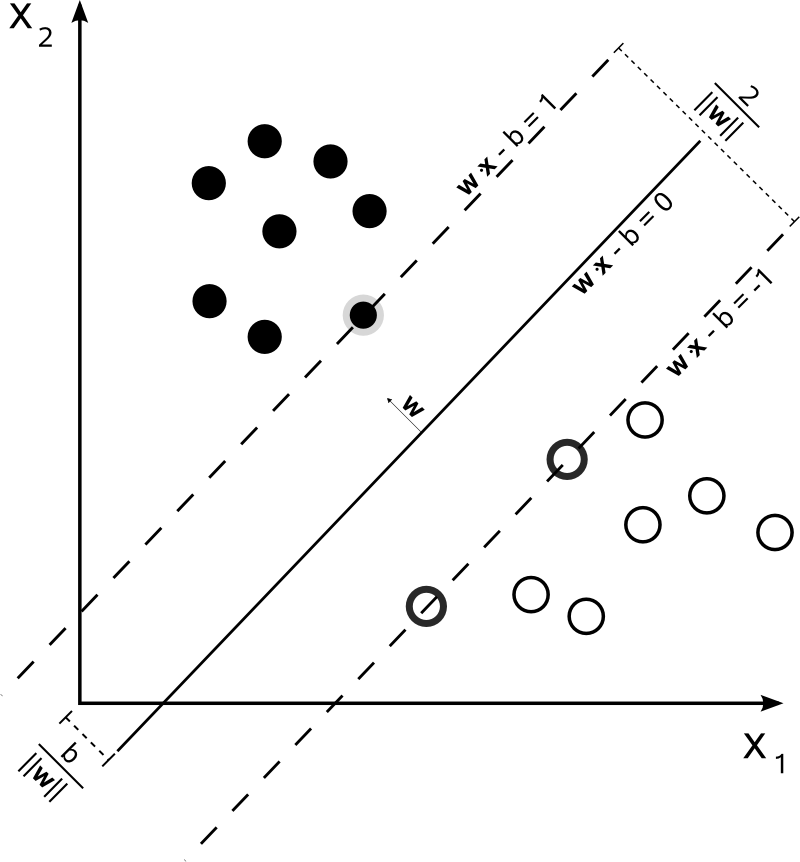
\includegraphics{D:/R-Intro/R-Intro/Lab-07/images/img1.png}
\caption{``Mo ta SVM''}
\end{figure}

Đường thẳng ``tốt nhất'' là đường có \textbf{lề (margin) lớn nhất} - tức
là khoảng cách từ đường đến các điểm dữ liệu gần nhất của mỗi lớp là lớn
nhất.

\end{document}
